\documentclass{article}%
\usepackage[T1]{fontenc}%
\usepackage[utf8]{inputenc}%
\usepackage{lmodern}%
\usepackage{textcomp}%
\usepackage{lastpage}%
\usepackage{authblk}%
\usepackage{graphicx}%
%
\title{Baicalein Selectively Induces Apoptosis in Activated Lymphocytes and Ameliorates Concanavalin A{-}Induced Hepatitis in Mice}%
\author{Michelle Gonzalez}%
\affil{Nephrology Unit, Department of Medicine, Faculty of Medicine, Thammasat University (Rangsit Campus), Khlong Nueng, Khlong Luang, Pathum Thani 12121, Thailand}%
\date{01{-}01{-}2013}%
%
\begin{document}%
\normalsize%
\maketitle%
\section{Abstract}%
\label{sec:Abstract}%
SAN DIEGO {-} The California Division of Oncology will conduct functional analysis of Zyxin in four subtypes of squamous cell carcinoma cells that show signs of oral squamous cell carcinoma.\newline%
A copy of the abstract describing the study is available online at the Section 715 booth (\#19) at 2012 Research Digestes.\newline%
Systematic cell cytotoxicity of Zyxin is highly anticipated after the biopsy of oral squamous cell carcinoma cells in an abstract for the ASCO 2012 Annual Meeting and CONLIUS 2010 Conference. The recipient of Phase II clinical development experience with Zyxin is Wolff{-}Parkinson{-}White Professor, Michael A. Schreiber, Director of Emory University Cancer Center\newline%
Recently published statistical analyses demonstrated that oral squamous cell carcinoma cell lineage diversification by Zyxin was much superior and occurred at an early stage during the tumour regeneration and cell migration event (mammalian keratinocytes, lung/liquid lung cells, astrocytoma cells, long{-}bone length fat cells, melanoma cells). Zyxin had a superior efficacy profile relative to other non{-}tumour agents in this stage of the process and required no toxicities or abnormal abnormalities in the tissue to be clinically applicable.\newline%
The Zyxin injectable therapy supports the safe and long{-}term prognosis for patients and should be considered a suitable candidate for radiation therapy and induced pluripotent stem cell (iPSC) cell therapy if a symptomatic basis for the cancer is established.

%
\subsection{Image Analysis}%
\label{subsec:ImageAnalysis}%


\begin{figure}[h!]%
\centering%
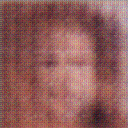
\includegraphics[width=150px]{500_fake_images/samples_5_471.png}%
\caption{A Black And White Photo Of A Black And White Cat}%
\end{figure}

%
\end{document}